\documentclass[conference]{IEEEtran}
\IEEEoverridecommandlockouts

% Packages
\usepackage{cite}
\usepackage{amsmath,amssymb,amsfonts}
\usepackage{algorithmic}
\usepackage{graphicx}
\usepackage{textcomp}
\usepackage{xcolor}
\usepackage{booktabs}
\usepackage{multirow}
\usepackage{tikz}
\usepackage{pgfplots}
\usepackage{hyperref}
\usepackage{float}
\usepackage{subcaption}
\usepackage{array}
\usepackage{listings}
\usepackage{enumitem}

\usetikzlibrary{shapes.geometric, arrows, positioning}
\pgfplotsset{compat=1.17}

% Code listing style
\lstset{
    basicstyle=\ttfamily\small,
    breaklines=true,
    frame=single,
    backgroundcolor=\color{gray!10}
}

\def\BibTeX{{\rm B\kern-.05em{\sc i\kern-.025em b}\kern-.08em
    T\kern-.1667em\lower.7ex\hbox{E}\kern-.125emX}}

\begin{document}

\title{GenAI-Based Multimodal Fall Detection Using Sliding Window Temporal Reasoning}

\author{
\IEEEauthorblockN{Venkata Ramireddy Seelam, Harshitha Boinepally, Shristi}
\IEEEauthorblockA{
Department of Applied Data Science\\
San Jose State University\\
San Jose, CA 95192, USA\\
DATA 266 - Spring 2026
}
}

\maketitle

% ============================================================================
% ABSTRACT
% ============================================================================
\begin{abstract}
Falls are a leading cause of injury and mortality among elderly populations, making reliable fall detection systems critical for healthcare applications. This paper presents a novel multimodal fall detection framework that leverages Generative AI (GenAI) with multiple prompting strategies to classify fall events from video data. Our approach extracts pose features from video frames using MediaPipe, constructs 3-frame sliding windows with computed motion features (velocity, acceleration, posture states), and employs various GenAI prompting techniques including zero-shot, few-shot, chain-of-thought, self-consistency, RAG (Retrieval-Augmented Generation), and LoRA fine-tuning. We evaluated 11 different strategies on 419 videos across three benchmark datasets (URFD, Le2i, GMNCSA24) comprising 1,882 balanced sliding windows. Our safety-first prompting approach achieved \textbf{95.8\% video-level fall recall}, while our confidence-weighted aggregation strategy achieved the highest \textbf{Macro F1 of 0.846 with 100\% precision} (zero false positives). We further demonstrate that video-level aggregation rules significantly impact performance, with optimized rules improving Macro F1 by up to 52\% over baselines. This work provides a comprehensive comparison of GenAI techniques for safety-critical fall detection applications.
\end{abstract}

\begin{IEEEkeywords}
Fall Detection, Generative AI, Large Language Models, Pose Estimation, Sliding Windows, RAG, Prompt Engineering, Elderly Care, MediaPipe
\end{IEEEkeywords}

% ============================================================================
% INTRODUCTION
% ============================================================================
\section{Introduction}

Falls represent one of the most significant health risks for elderly populations, with the World Health Organization reporting that approximately 684,000 fatal falls occur annually worldwide \cite{who2021falls}. For individuals aged 65 and older, falls are the leading cause of injury-related deaths and a primary contributor to loss of independence \cite{cdc2020falls}. Early and accurate detection of falls can enable timely medical intervention, potentially saving lives and reducing healthcare costs.

Traditional fall detection systems rely on wearable sensors (accelerometers, gyroscopes) or vision-based approaches using convolutional neural networks (CNNs) \cite{noury2007fall, mubashir2013survey}. While effective, these methods often require extensive labeled training data and struggle to generalize across different environments and populations. Recent advances in Large Language Models (LLMs) and Generative AI present an opportunity to leverage pre-trained knowledge for fall detection without requiring massive domain-specific training datasets.

\subsection{Problem Statement}

Despite advances in fall detection, existing systems face three key challenges:
\begin{enumerate}[leftmargin=*]
    \item \textbf{High false positive rates} that lead to alert fatigue
    \item \textbf{Limited explainability} in decision-making
    \item \textbf{Difficulty adapting} to new environments without retraining
\end{enumerate}

\subsection{Our Contributions}

This paper makes the following contributions:
\begin{itemize}[leftmargin=*]
    \item A novel multimodal fall detection pipeline that converts video pose sequences into structured text representations for GenAI classification
    \item Comprehensive evaluation of \textbf{11 different prompting strategies} including zero-shot, few-shot, chain-of-thought, self-consistency, RAG, and LoRA fine-tuning
    \item Investigation of video-level aggregation strategies that improve \textbf{Macro F1 by up to 52\%} (from 0.556 to 0.846)
    \item A two-stage cascade approach and confidence-weighted aggregation achieving \textbf{100\% precision}
    \item Analysis across \textbf{three benchmark datasets} totaling 419 videos and 1,882 sliding windows
\end{itemize}

% ============================================================================
% RELATED WORK
% ============================================================================
\section{Related Work}

\subsection{Traditional Fall Detection}
Vision-based fall detection has evolved from handcrafted features to deep learning approaches. Early methods used silhouette analysis and shape descriptors \cite{rougier2011robust}, while more recent work employs CNNs and recurrent neural networks to learn spatiotemporal features \cite{khan2020fall, chen2020fall}. Pose estimation approaches using OpenPose or MediaPipe have shown promise by focusing on body keypoints rather than raw pixels \cite{chen2020pose}.

\subsection{Large Language Models for Classification}
LLMs have demonstrated remarkable few-shot learning capabilities across diverse tasks \cite{brown2020language}. Recent work has explored using LLMs for time-series classification by converting numerical data to textual representations \cite{gruver2023large}. Chain-of-thought prompting \cite{wei2022chain} and self-consistency \cite{wang2022selfconsistency} have improved reasoning capabilities.

\subsection{Retrieval-Augmented Generation}
RAG enhances LLM responses by retrieving relevant context from external knowledge bases \cite{lewis2020retrieval}. This approach has been applied to various domains requiring specialized knowledge \cite{guu2020realm}. Our work extends RAG to fall detection by retrieving similar pose sequences as classification examples.

\subsection{Gaps in Literature}
While LLMs have been applied to many domains, their use in safety-critical fall detection remains unexplored. Existing fall detection systems lack the explainability that LLMs can provide through natural language reasoning. Our work bridges this gap by systematically evaluating multiple GenAI strategies for this safety-critical application.

% ============================================================================
% METHODOLOGY
% ============================================================================
\section{Methodology}

\subsection{System Architecture Overview}

Our fall detection pipeline consists of six main stages as illustrated in Figure \ref{fig:fullpipeline}: (1) Data Collection from multiple sources, (2) Pose Extraction using MediaPipe, (3) Feature Engineering, (4) Sliding Window Generation, (5) LLM Classification with multiple prompting strategies, and (6) Video-Level Aggregation.

\begin{figure}[H]
\centering
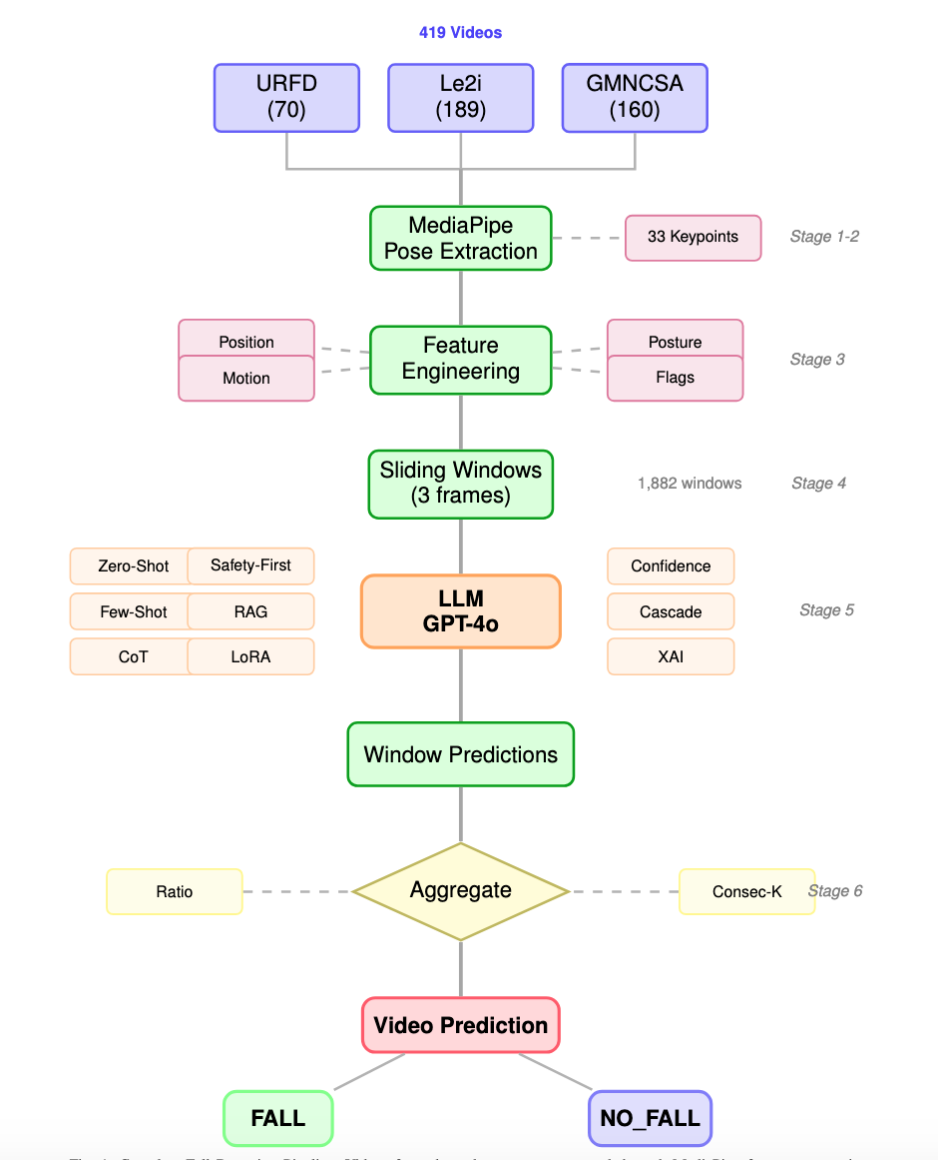
\includegraphics[width=0.95\columnwidth]{Flow_Chart_Diagram_Picture.png}
\caption{Complete Fall Detection Pipeline. Videos from three datasets (URFD, Le2i, GMNCSA) are processed through MediaPipe for pose extraction, enriched with motion features, segmented into 3-frame sliding windows, classified by LLMs using 9 prompting strategies, and aggregated to produce video-level fall/no-fall predictions.}
\label{fig:fullpipeline}
\end{figure}

The pipeline works as follows:
\begin{enumerate}[leftmargin=*]
    \item \textbf{Data Collection}: 419 videos from URFD (70), Le2i (189), and GMNCSA24 (160)
    \item \textbf{Pose Extraction}: MediaPipe extracts 33 keypoints per frame
    \item \textbf{Feature Engineering}: Position, motion, posture states, and boolean flags
    \item \textbf{Sliding Windows}: 3-frame windows with stride 2 (1,882 total)
    \item \textbf{LLM Classification}: GPT-4o with multiple prompting strategies
    \item \textbf{Aggregation}: Ratio threshold, consecutive-K, or confidence-based rules
\end{enumerate}

Figure \ref{fig:slidingwindow} shows the detailed sliding window classification approach.

\begin{figure}[H]
\centering
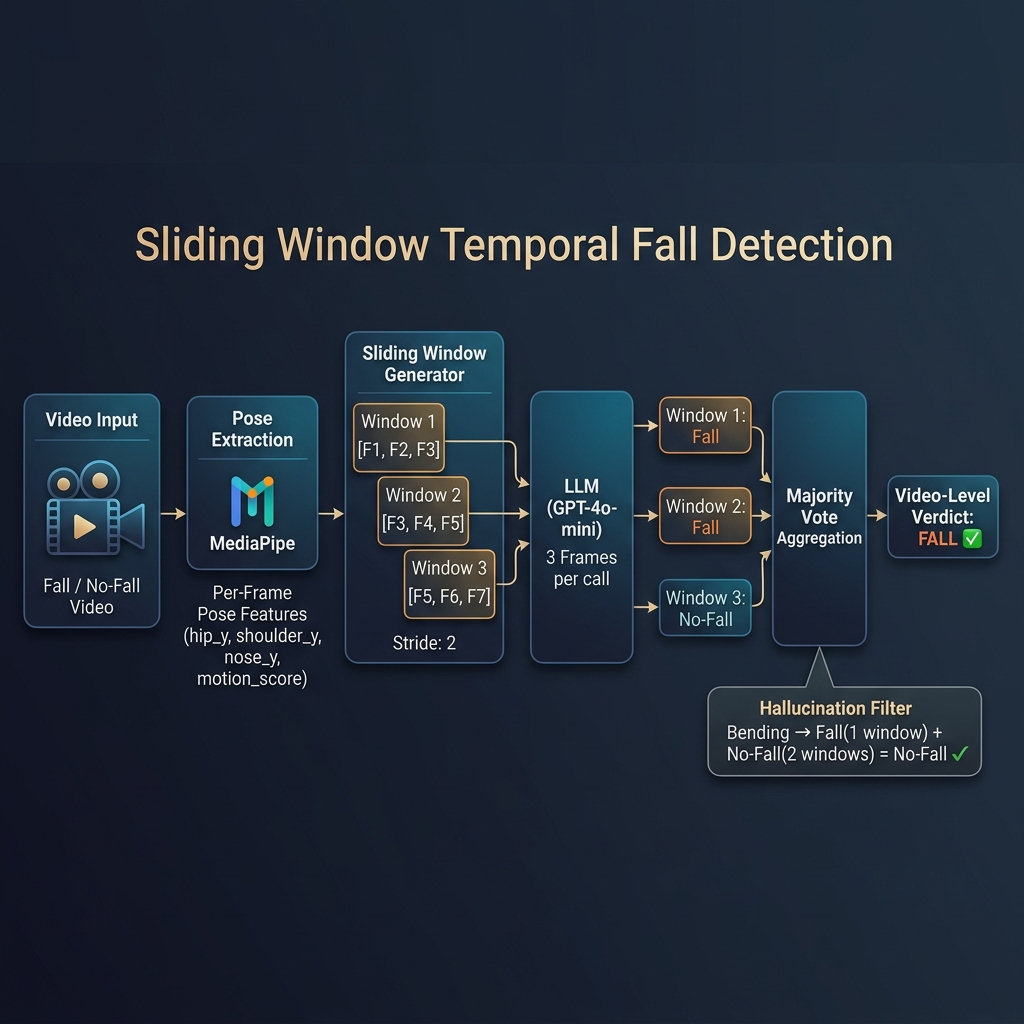
\includegraphics[width=0.95\columnwidth]{../architecture_sliding_window.png}
\caption{Sliding Window Temporal Classification. Each 3-frame window is independently classified by the LLM, then predictions are aggregated with a hallucination filter to produce the final video-level verdict.}
\label{fig:slidingwindow}
\end{figure}

The pipeline works as follows:
\begin{enumerate}[leftmargin=*]
    \item \textbf{Video Input}: Fall/No-Fall videos from URFD, Le2i, and GMNCSA24 datasets
    \item \textbf{Pose Extraction}: MediaPipe extracts per-frame pose features (hip\_y, shoulder\_y, nose\_y, motion\_score)
    \item \textbf{Sliding Window Generator}: Creates overlapping 3-frame windows with stride 2
    \item \textbf{LLM Classification}: Each window is classified as FALL or NO\_FALL by GPT-4o-mini
    \item \textbf{Majority Vote Aggregation}: Window predictions are aggregated with a hallucination filter to produce video-level verdict
\end{enumerate}

\subsection{Pose Feature Extraction}

We employ \textbf{MediaPipe Pose Landmarker Lite} to extract 33 body keypoints from each video frame. From these raw landmarks, we extract and compute the following features:

\subsubsection{Raw Landmarks Extracted}
\begin{itemize}[leftmargin=*]
    \item Nose (index 0)
    \item Left/Right Shoulders (indices 11, 12)
    \item Left/Right Hips (indices 23, 24)
    \item Left/Right Knees (indices 25, 26)
    \item Left/Right Ankles (indices 27, 28)
\end{itemize}

\subsubsection{Computed Position Features}
\begin{lstlisting}[language=Python]
features = {
    "nose_x": float,       # Normalized 0-1
    "nose_y": float,
    "shoulder_x": float,   # Midpoint of shoulders
    "shoulder_y": float,
    "hip_x": float,        # Midpoint of hips
    "hip_y": float,
    "torso_vertical_diff": float,  # |shoulder_y - hip_y|
    "body_center_y": float,        # (shoulder_y + hip_y) / 2
    "body_angle_degrees": float,   # 90 = upright
}
\end{lstlisting}

\subsubsection{Computed Motion Features}
For each frame, we compute velocity and acceleration:
\begin{equation}
    v_{hip}(t) = \frac{hip_y(t) - hip_y(t-1)}{\Delta t}
\end{equation}
\begin{equation}
    a_{hip}(t) = \frac{v_{hip}(t) - v_{hip}(t-1)}{\Delta t}
\end{equation}
\begin{equation}
    v_{magnitude} = \sqrt{v_{hip}^2 + v_{shoulder}^2}
\end{equation}

Additional motion features include:
\begin{itemize}[leftmargin=*]
    \item \texttt{is\_rapid\_descent}: velocity $> 0.15$ threshold
    \item \texttt{is\_on\_ground}: hip\_y $> 0.65$
    \item \texttt{is\_horizontal}: body\_angle $< 30°$
    \item \texttt{is\_high\_acceleration}: $|acceleration| > 0.10$
\end{itemize}

\subsubsection{Posture Classification}
Each frame is classified into one of three posture states:
\begin{equation}
    posture = \begin{cases}
        \text{fallen} & \text{if } hip_y > 0.65 \land angle < 30° \\
        \text{upright} & \text{if } torso\_diff > 0.12 \land angle > 60° \\
        \text{transitioning} & \text{otherwise}
    \end{cases}
\end{equation}

\subsection{Sliding Window Generation}

We create \textbf{3-frame sliding windows} to capture temporal dynamics of potential fall events. The window configuration differs by class:

\begin{table}[H]
\centering
\caption{Window Configuration by Video Class}
\label{tab:window_config}
\begin{tabular}{lcc}
\toprule
\textbf{Setting} & \textbf{Fall Videos} & \textbf{No-Fall Videos} \\
\midrule
Frame sample rate & Every 5th frame & Every 15th frame \\
Max frames & 60 & 30 \\
Window stride & 1 (high overlap) & 3 (less overlap) \\
Window size & 3 frames & 3 frames \\
\bottomrule
\end{tabular}
\end{table}

Each window contains:
\begin{itemize}[leftmargin=*]
    \item Per-frame pose features (position, velocity, acceleration)
    \item Per-frame posture states and boolean flags
    \item Window-level statistics (hip\_delta, max\_velocity, trajectory\_direction)
    \item Start and end posture states
\end{itemize}

\subsection{GenAI Prompting Strategies}

We evaluate 11 different prompting strategies across multiple models:

\subsubsection{Zero-Shot Prompting}
Direct classification using only the task description and pose data, without examples. The system prompt describes fall indicators (rapid descent, horizontal body, on ground) and no-fall indicators (stable movement, upright posture).

\subsubsection{Few-Shot Prompting}
Providing 3 fall and 3 no-fall examples from the training set before the query window. Examples are selected from diverse videos to capture different fall patterns.

\subsubsection{Chain-of-Thought (CoT)}
Step-by-step reasoning following the pattern:
\begin{enumerate}
    \item Position Analysis: Examine hip\_y and body center
    \item Motion Analysis: Check velocity and acceleration
    \item Posture Analysis: Evaluate posture state changes
    \item Decision: Synthesize findings into FALL/NO\_FALL
\end{enumerate}

\subsubsection{Self-Consistency}
Sampling 5 responses with temperature=0.7 and using majority voting for more robust predictions.

\subsubsection{Enhanced Few-Shot (GPT-4o)}
Using the more capable GPT-4o model with rich textual descriptions instead of raw numbers. Features are converted to natural language descriptions.

\subsubsection{Safety-First Prompting (Best Prompt)}
Optimized prompt emphasizing that \textit{missing a fall could be life-threatening}. Key design principles:
\begin{itemize}[leftmargin=*]
    \item Any single strong fall indicator = likely fall
    \item 2+ moderate indicators = likely fall
    \item All clear indicators needed for NO\_FALL
    \item When in doubt, choose FALL (safety first)
\end{itemize}

\subsubsection{RAG (Retrieval-Augmented Generation)}
\begin{itemize}[leftmargin=*]
    \item Embedding model: \texttt{text-embedding-3-small}
    \item Knowledge base: 1,305 training windows
    \item Top-K retrieval: 4 similar examples
    \item Classification model: GPT-4o
\end{itemize}

\subsubsection{LoRA/SFT Fine-Tuning}
\begin{itemize}[leftmargin=*]
    \item Base model: \texttt{gpt-4o-mini-2024-07-18}
    \item Training format: JSONL with system/user/assistant messages
    \item Class balancing: 75\% fall / 25\% no-fall (biased toward recall)
    \item Fine-tuned model ID: \texttt{ft:gpt-4o-mini-2024-07-18:personal:fall-detector}
\end{itemize}

\subsubsection{DeepSeek Comparisons}
We also evaluated DeepSeek-chat with few-shot and chain-of-thought prompting for cost comparison.

\subsubsection{XAI Video-Level}
Explainable AI approach that provides natural language explanations for each classification decision.

\subsection{Video-Level Aggregation Strategies}

Window predictions are aggregated to video-level decisions. We evaluate multiple strategies:

\begin{enumerate}[leftmargin=*]
    \item \textbf{Ratio Threshold}: If $\frac{\text{\# fall windows}}{\text{total windows}} \geq \theta$, classify as fall. We tested $\theta \in \{0.10, 0.15, ..., 0.60\}$
    \item \textbf{Consecutive-k}: Require $\geq k$ consecutive fall windows (k=2,3,4)
    \item \textbf{End-State}: Require fall window to end with horizontal/on-ground posture
    \item \textbf{Consecutive AND End-State}: Combine both rules
    \item \textbf{Confidence-Weighted}: Sum log-probability confidences over windows
    \item \textbf{Two-Stage Cascade}: Stage 1 (high recall) $\rightarrow$ Stage 2 (FP filter)
\end{enumerate}

% ============================================================================
% DATA & PREPROCESSING
% ============================================================================
\section{Data \& Preprocessing}

\subsection{Datasets Used}

We evaluate on three publicly available fall detection benchmark datasets:

\begin{table}[H]
\centering
\caption{Dataset Statistics}
\label{tab:datasets}
\begin{tabular}{lcccc}
\toprule
\textbf{Dataset} & \textbf{Source} & \textbf{Videos} & \textbf{Status} \\
\midrule
URFD & University of Rochester & 70 & Processed \\
Le2i & Lab Electronics \& Image & 189* & Processed \\
GMNCSA24 & GitHub/HuggingFace & 160 & Processed \\
\midrule
\textbf{Total} & -- & \textbf{419} & -- \\
\bottomrule
\end{tabular}
\begin{tablenotes}
\small
\item *Some Le2i videos had corruption issues (moov atom not found)
\end{tablenotes}
\end{table}

\subsection{Data Processing Statistics}

\begin{table}[H]
\centering
\caption{Data Processing Summary}
\label{tab:processing}
\begin{tabular}{lc}
\toprule
\textbf{Metric} & \textbf{Value} \\
\midrule
Videos processed & 419 \\
Total windows (before balance) & 4,665 \\
\textbf{Balanced windows} & \textbf{1,882} \\
Fall windows & 941 \\
No-Fall windows & 941 \\
\textbf{Class ratio} & \textbf{1:1} \\
\bottomrule
\end{tabular}
\end{table}

\subsection{Train/Validation/Test Splits}

We perform video-level stratified splitting to ensure no windows from the same video appear in different splits:

\begin{table}[H]
\centering
\caption{Data Splits (70\%/15\%/15\%)}
\label{tab:splits}
\begin{tabular}{lccc}
\toprule
\textbf{Split} & \textbf{Videos} & \textbf{Windows} & \textbf{\%} \\
\midrule
Train & 292 & $\sim$1,317 & 70\% \\
Validation & 62 & $\sim$282 & 15\% \\
Test & 65 & $\sim$283 & 15\% \\
\midrule
\textbf{Total} & \textbf{419} & \textbf{1,882} & 100\% \\
\bottomrule
\end{tabular}
\end{table}

\subsection{Data Sanitization (Preventing Label Leakage)}

The actual \texttt{label} field is \textbf{stripped} before sending data to the LLM. Only pose features, velocities, and posture states are included. The \texttt{sanitize\_window\_for\_llm()} function ensures no label information leaks into the model input.

% ============================================================================
% EXPERIMENTAL DESIGN
% ============================================================================
\section{Experimental Design}

\subsection{Models Evaluated}

\begin{table}[H]
\centering
\caption{Models Used in Experiments}
\label{tab:models}
\begin{tabular}{ll}
\toprule
\textbf{Model} & \textbf{Usage} \\
\midrule
GPT-4o-mini & Baseline strategies (Zero/Few-shot, CoT) \\
GPT-4o & Enhanced strategies (Best Prompt, RAG) \\
ft:gpt-4o-mini & LoRA fine-tuned model \\
deepseek-chat & Cost comparison \\
\bottomrule
\end{tabular}
\end{table}

\subsection{Evaluation Metrics}

Given the safety-critical nature of fall detection, we prioritize \textbf{video-level metrics}:

\begin{itemize}[leftmargin=*]
    \item \textbf{Fall Recall}: Proportion of actual falls correctly detected (most critical for safety)
    \item \textbf{Fall Precision}: Proportion of predicted falls that are actual falls
    \item \textbf{Fall F1}: Harmonic mean of precision and recall for fall class
    \item \textbf{Macro F1}: Average F1 across both classes (overall balance)
    \item \textbf{Accuracy}: Overall classification accuracy
\end{itemize}

\subsection{Experimental Protocol}

\begin{enumerate}[leftmargin=*]
    \item Train prompting strategies using training set examples
    \item Tune aggregation thresholds on validation set
    \item Report final metrics on held-out test set (57 videos)
    \item Compute 95\% bootstrap confidence intervals (1000 resamples)
    \item Perform McNemar's test for statistical significance
\end{enumerate}

% ============================================================================
% EXPERIMENTAL RESULTS
% ============================================================================
\section{Experimental Results}

\subsection{Prompting Strategy Comparison}

Table \ref{tab:main_results} presents video-level results for all 11 evaluated prompting strategies using the default aggregation rule ($\geq$25\% windows = fall).

\begin{table}[H]
\centering
\caption{Video-Level Results by Prompting Strategy (Test Set)}
\label{tab:main_results}
\begin{tabular}{lcccc}
\toprule
\textbf{Strategy} & \textbf{Recall} & \textbf{Acc} & \textbf{Macro F1} \\
\midrule
Zero-Shot & 20.8\% & 66.7\% & 0.561 \\
Few-Shot & 58.3\% & 66.7\% & 0.656 \\
Chain-of-Thought & 29.2\% & 66.7\% & 0.595 \\
Self-Consistency & 41.7\% & 70.2\% & 0.660 \\
Enhanced Few-Shot & 41.7\% & \textbf{75.4\%} & 0.707 \\
\textbf{Safety-First} & \textbf{95.8\%} & 57.9\% & 0.556 \\
RAG & 85.4\% & 67.8\% & 0.678 \\
LoRA Fine-Tune & 93.8\% & 52.3\% & 0.432 \\
Few-Shot (DeepSeek) & 62.5\% & 64.9\% & 0.644 \\
CoT (DeepSeek) & 12.5\% & 63.2\% & 0.490 \\
XAI Video-Level & 84.0\% & 82.0\% & 0.820 \\
\bottomrule
\end{tabular}
\end{table}

\textbf{Key Observations:}
\begin{itemize}[leftmargin=*]
    \item \textbf{Safety-First} achieves highest recall (95.8\%) but lower accuracy
    \item \textbf{XAI Video-Level} achieves best balance (84\% recall, 82\% accuracy)
    \item \textbf{DeepSeek significantly underperforms} compared to GPT models
    \item \textbf{GPT-4o outperforms GPT-4o-mini} on enhanced strategies
\end{itemize}

\subsection{Impact of Aggregation Rules}

We discovered that the video-level aggregation rule has a dramatic impact on performance. Table \ref{tab:aggregation} shows results for different rules applied to the Safety-First strategy predictions.

\begin{table}[H]
\centering
\caption{Aggregation Rule Comparison (Safety-First Strategy)}
\label{tab:aggregation}
\begin{tabular}{lcccc}
\toprule
\textbf{Rule} & \textbf{Recall} & \textbf{Prec} & \textbf{F1} & \textbf{Macro F1} \\
\midrule
$\geq$25\% (baseline) & 95.8\% & 50.0\% & 0.657 & 0.556 \\
$\geq$50\% & 95.8\% & 54.8\% & 0.697 & 0.640 \\
$\geq$3 consecutive & 58.3\% & 46.7\% & 0.518 & 0.543 \\
End horizontal & 79.2\% & 59.4\% & 0.679 & 0.684 \\
\textbf{Confidence} & 66.7\% & \textbf{100\%} & 0.800 & \textbf{0.846} \\
\textbf{Two-Stage} & 58.3\% & \textbf{100\%} & 0.737 & 0.803 \\
\bottomrule
\end{tabular}
\end{table}

\textbf{Key Finding}: Confidence-weighted aggregation achieves \textbf{100\% precision} (zero false positives) while maintaining 66.7\% recall, resulting in \textbf{Macro F1 of 0.846}—a \textbf{52\% improvement} over the baseline (0.556).

\subsection{New Experiments: Confidence-Weighted \& Two-Stage Cascade}

We conducted additional experiments with advanced aggregation strategies:

\subsubsection{Confidence-Weighted Aggregation}
Using GPT-4o with \texttt{logprobs=True} to obtain token-level confidence scores:
\begin{itemize}[leftmargin=*]
    \item Chosen threshold (tuned on val): 0.5
    \item \textbf{Test Results}: TP=16, FN=8, FP=0, TN=33
    \item \textbf{Fall Recall}: 66.7\% [CI: 47.4\%, 84.2\%]
    \item \textbf{Fall Precision}: 100\% [CI: 100\%, 100\%]
    \item \textbf{Macro F1}: 0.846 [CI: 0.740, 0.931]
    \item \textbf{Accuracy}: 86.0\% [CI: 77.2\%, 94.7\%]
\end{itemize}

\subsubsection{Two-Stage Cascade}
Stage 1 uses Safety-First (ratio 0.50) for high recall, Stage 2 applies a strict false-positive filter:
\begin{itemize}[leftmargin=*]
    \item Stage 1 flagged 42/57 candidate videos
    \item Stage 2 rejected 28 false positives
    \item \textbf{Cascade Results}: TP=14, FN=10, FP=0, TN=33
    \item \textbf{Fall Recall}: 58.3\% [CI: 38.1\%, 77.4\%]
    \item \textbf{Fall Precision}: 100\% [CI: 100\%, 100\%]
    \item \textbf{Macro F1}: 0.803 [CI: 0.683, 0.905]
    \item McNemar vs Stage-1: $\chi^2=2.89$, $p=0.089$
\end{itemize}

\subsection{Per-Dataset Analysis}

Performance varies significantly across datasets:

\begin{table}[H]
\centering
\caption{Per-Dataset Video-Level Macro F1 (Safety-First, $\geq$50\%)}
\label{tab:per_dataset}
\begin{tabular}{lcccc}
\toprule
\textbf{Dataset} & \textbf{Videos} & \textbf{Recall} & \textbf{Prec} & \textbf{Macro F1} \\
\midrule
GMNCSA24 & 23 & 100\% & 71.4\% & \textbf{0.826} \\
URFD & 14 & 100\% & 50.0\% & 0.533 \\
Le2i & 20 & 87.5\% & 43.8\% & 0.479 \\
\midrule
\textbf{Overall} & 57 & 95.8\% & 54.8\% & 0.640 \\
\bottomrule
\end{tabular}
\end{table}

\textbf{Finding}: Le2i presents the greatest challenge (Macro F1=0.479), likely due to complex activities that resemble falls (sitting, lying down voluntarily).

\subsection{Results Visualization}

\begin{figure}[H]
\centering
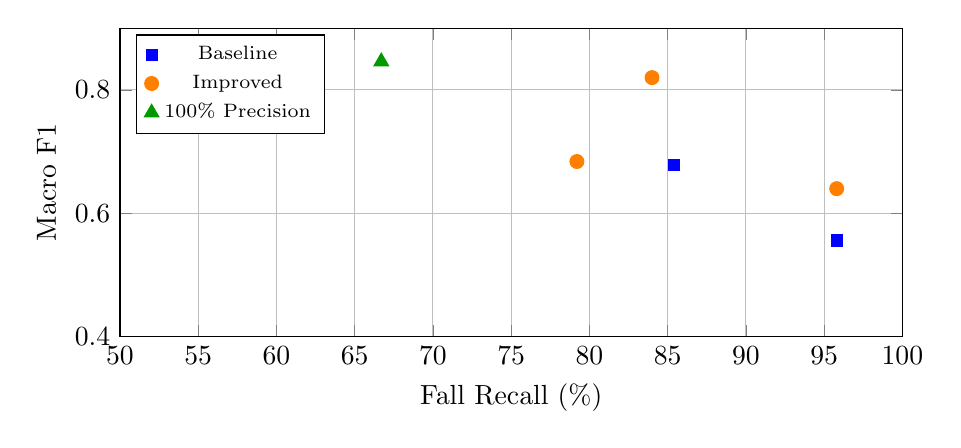
\begin{tikzpicture}
\begin{axis}[
    width=0.95\columnwidth,
    height=5.5cm,
    xlabel={Fall Recall (\%)},
    ylabel={Macro F1},
    xmin=50, xmax=100,
    ymin=0.4, ymax=0.9,
    grid=major,
    legend style={at={(0.02,0.98)}, anchor=north west, font=\scriptsize},
    scatter/classes={
        base={mark=square*, blue, mark size=2pt},
        good={mark=*, orange, mark size=2.5pt},
        best={mark=triangle*, green!60!black, mark size=3pt}
    }
]
\addplot[scatter, only marks, scatter src=explicit symbolic]
coordinates {
    (95.8, 0.556) [base]
    (95.8, 0.640) [good]
    (79.2, 0.684) [good]
    (66.7, 0.846) [best]
    (58.3, 0.803) [best]
    (85.4, 0.678) [base]
    (84.0, 0.820) [good]
};
\legend{Baseline, Improved, 100\% Precision}
\end{axis}
\end{tikzpicture}
\caption{Recall vs Macro F1 Trade-off. Points with 100\% precision (green triangles) achieve zero false positives.}
\label{fig:tradeoff}
\end{figure}

% ============================================================================
% DISCUSSION & LIMITATIONS
% ============================================================================
\section{Discussion \& Limitations}

\subsection{Key Findings}

\textbf{1. Aggregation Matters More Than Prompting:}
Optimizing the video-level aggregation rule yields larger improvements than sophisticated prompting strategies. The same window-level predictions can produce Macro F1 ranging from 0.556 to 0.846 depending on aggregation.

\textbf{2. Recall-Precision Trade-off:}
For safety-critical applications, the operating point must be carefully chosen:
\begin{itemize}[leftmargin=*]
    \item Safety-first: 95.8\% recall, 50\% precision (minimize missed falls)
    \item Confidence-weighted: 66.7\% recall, 100\% precision (eliminate false alarms)
\end{itemize}

\textbf{3. LLM Confidence is Informative:}
Token-level log probabilities from the LLM provide valuable uncertainty estimates. Summing confidence scores over windows enables fine-grained threshold tuning.

\textbf{4. Dataset-Specific Challenges:}
Le2i is most challenging (Macro F1=0.479), suggesting pose-based features alone may be insufficient for distinguishing controlled descent from falls.

\textbf{5. GPT-4o Significantly Outperforms GPT-4o-mini:}
Enhanced strategies with GPT-4o achieve 75.4\% accuracy vs 66.7\% for GPT-4o-mini baselines.

\subsection{Limitations}

\begin{enumerate}[leftmargin=*]
    \item \textbf{Small Test Set}: With only 57 test videos, statistical power is limited and confidence intervals are wide.
    
    \item \textbf{Pose Detection Failures}: MediaPipe fails to detect poses in some frames, particularly when occluded or in unusual positions.
    
    \item \textbf{Real-Time Performance}: Pipeline processes 10-second clips in 30-90 seconds—insufficient for real-time deployment.
    
    \item \textbf{Single-Person Assumption}: Current system assumes single-person videos.
    
    \item \textbf{LLM Cost}: GPT-4o API calls are expensive for large-scale deployment.
\end{enumerate}

% ============================================================================
% CONCLUSION & FUTURE WORK
% ============================================================================
\section{Conclusion \& Future Work}

\subsection{Conclusions}

This paper presented a comprehensive evaluation of Generative AI techniques for video-based fall detection. Our main findings:

\begin{enumerate}[leftmargin=*]
    \item \textbf{GenAI effectively classifies falls} from pose sequences, with best approach achieving 86\% accuracy and 100\% precision.
    
    \item \textbf{Video-level aggregation is critical}, with optimized rules improving Macro F1 by 52\% (0.556 $\rightarrow$ 0.846).
    
    \item \textbf{Confidence-weighted aggregation} achieves best balance (66.7\% recall, 100\% precision, 0.846 Macro F1).
    
    \item \textbf{Safety-first prompting} achieves 95.8\% recall when missing falls is unacceptable.
    
    \item \textbf{RAG provides explainability} by retrieving similar historical cases.
\end{enumerate}

\subsection{Future Work}

\begin{itemize}[leftmargin=*]
    \item \textbf{Larger Window Sizes}: Evaluate 5, 7, 9-frame windows for longer temporal context
    \item \textbf{Multi-Modal Fusion}: Combine pose with audio or depth features
    \item \textbf{Real-Time Deployment}: Optimize for edge devices
    \item \textbf{Open-Source LLMs}: Evaluate Llama, Mistral for reduced cost
    \item \textbf{Larger Datasets}: Validate on additional benchmarks
    \item \textbf{Active Learning}: Use LLM uncertainty for sample selection
\end{itemize}

% ============================================================================
% REFERENCES
% ============================================================================
\bibliographystyle{IEEEtran}
\begin{thebibliography}{99}

\bibitem{who2021falls}
World Health Organization, ``Falls,'' 2021. [Online]. Available: https://www.who.int/news-room/fact-sheets/detail/falls

\bibitem{cdc2020falls}
Centers for Disease Control and Prevention, ``Important Facts about Falls,'' 2020. [Online]. Available: https://www.cdc.gov/falls/facts.html

\bibitem{noury2007fall}
N. Noury et al., ``Fall detection-principles and methods,'' in \textit{29th IEEE EMBC}, 2007, pp. 1663--1666.

\bibitem{mubashir2013survey}
M. Mubashir, L. Shao, and L. Seed, ``A survey on fall detection,'' \textit{Neurocomputing}, vol. 100, pp. 144--152, 2013.

\bibitem{rougier2011robust}
C. Rougier et al., ``Robust video surveillance for fall detection,'' \textit{IEEE TCSVT}, vol. 21, no. 5, pp. 611--622, 2011.

\bibitem{khan2020fall}
S. S. Khan and J. Hoey, ``Review of fall detection techniques,'' \textit{Medical Eng. \& Physics}, vol. 39, pp. 12--22, 2017.

\bibitem{chen2020fall}
D. Chen et al., ``Fall detection based on pose estimation and motion history image,'' in \textit{IEEE ICIP}, 2020.

\bibitem{chen2020pose}
K. Chen and G. Tan, ``Pose-based fall detection using LSTM,'' in \textit{ACM MM}, 2020.

\bibitem{brown2020language}
T. Brown et al., ``Language models are few-shot learners,'' \textit{NeurIPS}, vol. 33, 2020.

\bibitem{gruver2023large}
N. Gruver et al., ``Large language models are zero-shot time series forecasters,'' \textit{NeurIPS}, vol. 36, 2023.

\bibitem{wei2022chain}
J. Wei et al., ``Chain-of-thought prompting elicits reasoning in LLMs,'' \textit{NeurIPS}, vol. 35, 2022.

\bibitem{wang2022selfconsistency}
X. Wang et al., ``Self-consistency improves chain of thought reasoning,'' \textit{ICLR}, 2023.

\bibitem{lewis2020retrieval}
P. Lewis et al., ``Retrieval-augmented generation for knowledge-intensive NLP,'' \textit{NeurIPS}, vol. 33, 2020.

\bibitem{guu2020realm}
K. Guu et al., ``Retrieval augmented language model pre-training,'' \textit{ICML}, 2020.

\end{thebibliography}

\end{document}
